\documentclass{article}
\usepackage{arxiv}

\usepackage[utf8]{inputenc}
\usepackage[english, russian]{babel}
\usepackage[T1]{fontenc}
\usepackage{url}
\usepackage{booktabs}
\usepackage{amsfonts}
\usepackage{nicefrac}
\usepackage{microtype}
\usepackage{lipsum}
\usepackage{graphicx}
\usepackage{natbib}
\usepackage{doi}



\title{Итеративное улучшение тематической модели с обратной связью от пользователя}

\author{ Горбулев Алексей Ильич \\
	\texttt{gorbulev.ai@phystech.edu} \\
	\And
	Алексеев Василий Антонович \\
	\texttt{vasiliy.alekseyev@phystech.edu} \\
	\And
    Воронцов Константин Вячеславович \\
    \texttt{vokov@forecsys.ru} \\
}
\date{}

\renewcommand{\undertitle}{}
\renewcommand{\shorttitle}{Итеративное улучшение тематической модели с обратной связью от пользователя}

%%% Add PDF metadata to help others organize their library
%%% Once the PDF is generated, you can check the metadata with
%%% $ pdfinfo template.pdf
%%% \hypersetup{
%%% pdftitle={A template for the arxiv style},
%%% pdfsubject={q-bio.NC, q-bio.QM},
%%% pdfauthor={David S.~Hippocampus, Elias D.~Striatum},
%%% pdfkeywords={First keyword, Second keyword, More},
%%% }

\begin{document}
\maketitle

%%% термин «мусорная» взята из изначального задания, возможно, стоит изменить на стилистический нейтральный термин, но пока этого делать не стал, чтобы не нарушать изначальное задание

%%% some issues will be fixed later

\begin{abstract}
	В работе представлен метод тематического моделирования с использованием обратной связи от пользователя. Обратная связь заключается в определении принадлежности темы к одной из трёх категорий: релевантная, нерелевантная, «мусорная». Требуется использовать на каждой итерации пользовательскую разметку таким образом, чтобы сохранить существующие релевантные темы и выделить новые релевантные темы из нерелевантных и «мусорных» при существующей возможности. В работе предлагается решение с использованием библиотек тематического моделирования и регуляризаторов сглаживания и декоррелирования. Вычислительный эксперимент проводится на текстовой коллекции, основанной на новостях сайта Lenta.ru.
\end{abstract}

\keywords{Тематическое моделирование \and ARTM \and Обработка естественного языка  }

\section{Введение}
Одним из методов анализа текстов, который применяется в том числе в социологических исследованиях и активно развивается в последнее время, является тематическое моделирование. Тематическая модель помогает оценить вероятность принадлежности текста к каждой из предполагаемых тем. Именно вероятностное тематическое моделирование использовалось при исследовании распространения информации о пандемии COVID-19 в Хорватии \citep{pandemic2021}, освещения в средствах массовых информации Литвы климатических изменений \citep{climate2021}.

Однако задача построения вероятностной тематической модели имеет бесконечно много решений \citep{bigartm}, что предоставляет возможность с помощью различных регуляризаторов учесть особенности данных и тем самым создать модель, которая подходит именно под специфику данного набора текстов. В то же время, не все темы могут оказаться подходящими в контексте проводимого исследования, вследствие чего коллекция текстов, которые по содержанию могут быть релевантными, может уменьшиться за счёт документов, которые отнесены к нерелевантной теме, но тем не менее могут содержать важную информацию, что может сделать само исследование менее полным и менее качественным.

Целью данного исследования является построение обновляемой тематической модели с использованием обратной связи от пользователя, с помощью которой как можно большее число текстов было бы отнесено к релевантным темам. Обратная связь симулирует поведение пользователя, который относит каждую из тем к одной из трёх категорий: релевантные темы, нерелевантные темы и «мусорные» темы. На каждой итерации обновление модели основывается на пользовательской разметке таким образом, чтобы сохранить уже существующие релевантные темы, а из иных тем по возможности выделить новые релевантные темы, и уменьшить количество тем, которые не относятся ни к релевантным, ни к нерелевантным.

Объектом данного исследования являются методы тематического моделирования, алгоритмы пользовательской разметки тем и итеративного обновления моделей.

Для решения задачи используются в том числе и методы аддитивной регуляризации тематических моделей (ARTM), реализованные в библиотеках с открытым кодом \texttt{BigARTM} и \texttt{TopicNet}, которые включают в себя регуляризаторы декоррелирования и сглаживания. Именно подход ARTM способствует оптимизации моделей по сумме нескольких критериев \citep{artm}, что помогает учитывать особенности коллекции текстов и сделать саму модель более устойчивой. В качестве набора текстовых данных используется известная коллекция 20 Newsgroups, которая содержит около $18$ тысяч сообщений, разделённых по $20$ темам.

\section{Постановка задачи}

%%% возможно, постановка не совсем корректна и не совсем отображает глубину этой задачи

Пусть $A$ — коллекция текстов, $T_i$ — множество тем на итерации $i \in \mathbb{N}$, $T_i^1 \subset T_i$ — подмножество релевантных тем с точки зрения пользователя, $T_i^2 \subset T_i$ — подмножество нерелевантных тем с точки зрения пользователя, $T_i^3 \subset T_i$ — подмножество «мусорных» тем с точки зрения пользователя, при этом $T_i = \sqcup_{k = 1}^3 T_i^k$, $M_i$ — состояние модели на итерации $i$. Тогда итеративное улучшение модели $M_i$ состоит в построении модели $M_{i + 1}$, такой, чтобы множество тем $T_{i + 1}$ удовлетворяло следующим требованиям:

$$T_i^1 \subset T_{i + 1}^1, \ \left| T_{i + 1}^3 \right| \leq \left| T_i^3 \right|$$

Если $\left| T_i^3 \right| \leq K$, где $K$ — ограничение на количество «мусорных» тем, то тогда $M_{i + 1} = M_i$. Иначе строится новая модель $M_{i + 1}$.

Темой для документа $a \in A$ называется элемент $f(a) \in T_i$, определённый по правилу $$f(a) = \arg \max \limits_{k \in  \overline{1, |T_i|} M_i^k (a)}$$

Здесь $k$ отвечает за координату вектора $M_i (a)$, который представляет собой выход модели $M_i$.

\section{Вычислительный эксперимент}

%%% На данный момент есть только базовый вариант эксперимента
Целью данного вычислительного эксперимента является нахождение способа улучшения тематической модели.
После обучения базовой модели полученные темы распределяются пользователем на три категории: релевантные, нерелевантные, "мусорные".
Далее используется несколько метрик, в том числе разреженность.
%%% TODO: пока не упомняты когерентность, разреженность и другие важные метрики, но они будут важны для финального варианта.
Новая модель строится добавлением новых регуляризаторов и изменением параметров.
Сравнивается количество тем в каждой категории и новые значения метрик.

\subsection{Описание данных}

\texttt{Описан базовый вариант.}

Для обучения тематических моделей использовались новости, опубликованные на сайте Lenta.ru с $1$ января по $31$ марта $2002$ года.
Каждая из $5492$ новостей распределена по одной из $8$ макротем.
%%% Подробнее будет со временем

\subsection{Базовая модель}

В качестве базовой модели $M_0$ используется тематическая модель с регуляризатором декоррелирования, применяемым относительно слов, прошедших лемматизацию
Всего используется $50$ специальных тем и $1$ фоновая. При предобработке данных используются токенизация по словам, лемматизация с помощью пакета PyMorphy3, выделение биграмм, приведение к формату, совместимому с Vowpal Wabbit.
Далее используется тематическая модель $M_1$, использующая регуляризаторы декоррелирования и сглаживания как для лемматизированных слов, так и для биграмм.

%%% Кроме того, обязательно нужно про усреднение, но проблемы с запуском с разным значением seed

\subsection{Предварительные результаты}

Среди тем, предложенных базовой моделью, были выделены $27$ релевантных, $11$ нерелевантных и $12$ "мусорных" тем.
Добавление новых регуляризаторов декоррелирования и сглаживания как для лемматизированных слов, так и для биграмм, позволило выделить $3$ новые релевантные темы среди "мусорных".

\begin{figure}[h]
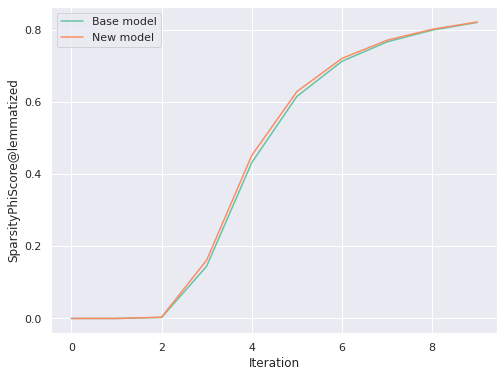
\includegraphics[width=9cm]{figures/sparsity_lemmatized.png}
\centering
\caption{Разреженность, лемматизированные слова}
\end{figure}

\begin{figure}[h]
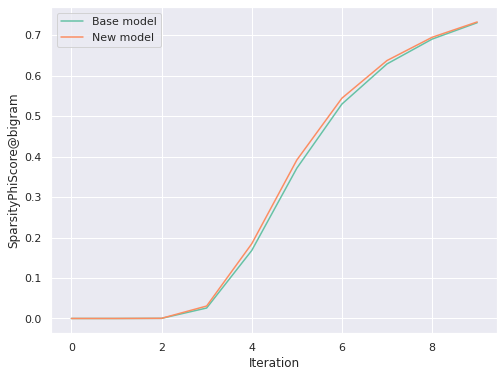
\includegraphics[width=9cm]
{figures/sparsity_bigram.png}
\centering
\caption{Разреженность, биграммы}
\end{figure}

Для новой модели разреженность выше, чем для базовой модели, что позволяет более точно определять темы с меньшим количеством возможных конфликтов.

\bibliographystyle{plain}
\bibliography{Gorbulev2023TopicModels}

\end{document}